%
% teil2.tex -- Beispiel-File für teil2
%
% (c) 2020 Prof Dr Andreas Müller, Hochschule Rapperswil
%
% !TEX root = ../../buch.tex
% !TEX encoding = UTF-8
%
\section{Kantorowitch-Formulierung%
\label{mongekant:section:teil2}}
\kopfrechts{Kantorowitch-Formulierung}

Im vorangegangenen Abschnitt haben wir das klassische Monge-Problem beschrieben.
Dieses Modell ist intuitiv,
aber die Forderung $T_{\#}\mu=\nu$ ist sehr streng.
Wie wir bereits in Abschnitt~\ref{mongekant:subsection:monge_inexistence} gesehen haben,
kann das Monge-Problem bereits für sehr einfache Masse keine Lösung besitzen.
Um dieses Existenzproblem zu umgehen,
hat Leonid Witaljewitch~Kantorowitch das Modell relaxiert.

\subsection{Transportpläne}
Statt nach einer Abbildung $T\colon X\to Y$ zu suchen,
führen wir einen \emph{Transportplan} $\gamma(x,y) \in \mathcal{P}(X \times Y)$ ein.
Hierbei ist $\mathcal{P}(X \times Y)$ die Menge aller Wahrscheinlichkeitsmasse
auf dem Produktraum $X \times Y$.
Der Plan $\gamma(x,y)$ gibt an,
wie viel Masse von $x \in X$ zu jedem Punkt $y \in Y$ transportiert wird.
Ein zulässiger Plan muss die Randbedingungen
\begin{align}
\begin{aligned}
\gamma(A \times Y)
&=
\mu(A)
,\quad \forall A \subset X
\\
\gamma(X \times B)
&=
\nu(B)
,\quad \forall B \subset Y
\end{aligned}
\label{mongekant:eq:kantorowitch_marginals}
\end{align}
erfüllen.
Die Menge aller zulässigen Transportpläne,
welche die Randbedingungen \eqref{mongekant:eq:kantorowitch_marginals} erfüllen,
bezeichnen wir mit $\Gamma(\mu, \nu)$.
Beispiele,
wie ein Transportplan aussehen kann,
sind in Abbildung~\ref{mongekant:fig:transport_plans} dargestellt.

\begin{figure}
\centering
\subfigure[{\color{red}Normal-} zu {\color{blue}Rayleigh-}Verteilung\label{mongekant:fig:plan1}]{
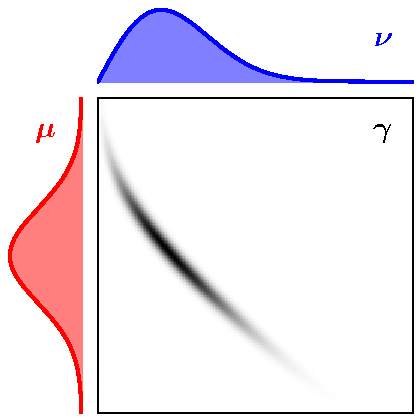
\includegraphics[width=0.48\textwidth]{papers/mongekant/code/ot_map_1}
}\hfill
\subfigure[{\color{red}Unimodal-} zu {\color{blue}Bimodal}verteilung\label{mongekant:fig:plan2}]{
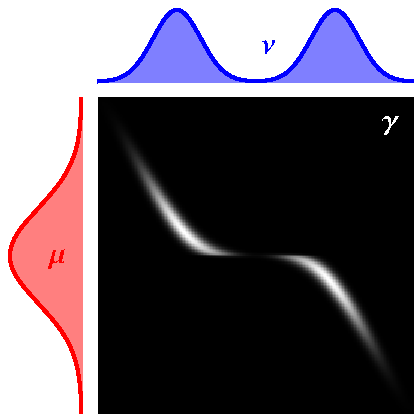
\includegraphics[width=0.48\textwidth]{papers/mongekant/code/ot_map_2}
}
\caption{Beispiele für Transportpläne $\gamma(x,y)$,
wobei $c(x,y) = |x - y|^2$ gewählt wurde.
Die Helligkeit ist an den Wert von $\gamma(x,y)$ ist.
Der Transportplan wurde hier für die bessere Sichtbarkeit noch zusätzlich geglättet.
}
\label{mongekant:fig:transport_plans}
\end{figure}

\subsection{Optimierungsproblem}
Mit diesen Transportplänen können wir das Optimierungsproblem zu 
\begin{align}
C_K(\mu, \nu)
&:=
\inf_{\gamma}
\int_{X \times Y} c(x,y)\, d\gamma(x,y)
,\quad
\forall \gamma \in \Gamma(\mu, \nu)
\label{mongekant:eq:kantorowitch_problem}
\end{align}
umformulieren.
Diese Umformulierung hat drei wesentliche Vorteile:
\begin{enumerate}
\item \textbf{Linearität.}
\eqref{mongekant:eq:kantorowitch_problem}
ist eine lineare Optimierung,
da sowohl die Zielfunktion
als auch die Randbedingungen \eqref{mongekant:eq:kantorowitch_marginals}
linear in $\gamma$ sind.
Hingegen ist das Monge-Problem \eqref{mongekant:eq:monge_problem}
stark nichtlinear in $T$.
\item \textbf{Existenz.}
Durch die Relaxation zu einer linearen Optimierung
über die konvexe Menge $\Gamma(\mu,\nu)$ kann man,
gemäss \cite{mongekant:ethlecture},
bereits unter sehr schwachen Annahmen
einen optimalen Plan $\gamma^{\ast}$ garantieren.
\item \textbf{Dualität.}
Das lineare Programm lässt sich in ein \emph{duales} Problem umformen,
was zu weiteren Einsichten in das Problem führt.
In Abschnitt~\ref{mongekant:subsection:kantorowitch_duality} werden
wir das duale Problem herleiten.
\end{enumerate}

\subsection{Zusammenhang zu Monge-Formulierung%
\label{mongekant:subsection:monge_kantorowitch_connection}}
Als nächstes wollen wir untersuchen,
wie die Monge- und Kantorowitch-Formulierung zusammenhängen und
ob sie ähnliche Ergebnisse liefern.
Dafür nehmen wir an,
dass eine Abbildung $T\colon X \to Y$ existiert,
für die \eqref{mongekant:eq:monge_problem} minimal wird.
Wählen wir jetzt
\begin{align}
d\gamma(x,y)
&=
d\mu(x) \delta_{y=T(x)}
\label{mongekant:eq:plan_from_map}
\end{align}
und setzen diesen Ausdruck
in die Randbedingungen \eqref{mongekant:eq:kantorowitch_marginals} ein,
\begin{align*}
\gamma(A \times Y)
&=
\int_A \delta_{T(x) \in Y}\, d\mu(x)
&
\gamma(X \times B)
&=
\int_X \delta_{T(x) \in B}\, d\mu(x)
\\
&=
\mu(A)
&&=
T_{\#}\mu\left(B\right)
\\
&&&=
\nu(B)
\end{align*}
sehen wir,
dass $\gamma(x,y)$ diese Bedingungen erfüllt.
Jetzt können wir also \eqref{mongekant:eq:plan_from_map} in
\eqref{mongekant:eq:kantorowitch_problem} einsetzen:
\begin{align*}
\int_{X \times Y} c(x,y)\, d\gamma(x,y)
&=
\int_X \int_Y c(x,y) \delta_{y=T(x)}\, dy\, d\mu(x)
\\
&=
\int_X c(x, T(x))\, d\mu(x)
.
\end{align*}
Das entpricht genau den Kosten in \eqref{mongekant:eq:monge_transport_cost}.
Daraus folgt,
\begin{align*}
C_K(\mu, \nu)
&\leq
C_M(\mu, \nu)
.
\end{align*}
Somit liefert die Kantorowitch-Formulierung immer mindestens so gute Ergebnisse
wie die Monge-Formulierung,
da jede Abbildung $T$ einen zulässigen Plan $\gamma$ definiert.
Berücksichtigt man zudem,
dass die Kantorowitch-Formulierung weniger strenge Anforderungen an das Problem stellt,
ergibt sich,
ein klarer Vorteil für die Kantorowitch-Formulierung.

\subsection{Dualität im Kantorowitch-Problem%
\label{mongekant:subsection:kantorowitch_duality}}

Um das duale Problem herzuleiten,
starten wir mit dem Kantorowitch-Problem \eqref{mongekant:eq:kantorowitch_problem}
und versuchen die Randbedingungen \eqref{mongekant:eq:kantorowitch_marginals}
mit Lagrange-Multiplikatoren $\xi \colon X \to \mathbb{R}$ und
$\eta \colon Y \to \mathbb{R}$ implizit in das Problem einzubauen,
so dass $\gamma$ nur noch eine Wahrscheinlichkeitsmass im Gebiet $X\times Y$ sein muss.
Dazu führen wir einen Langrange-Multiplikatorenterm $L(\xi,\eta)$ ein:
\begin{align*}
\begin{aligned}
C_K(\mu, \nu)
&=
\inf_{\gamma \in \Gamma} \int_{X \times Y} c(x,y)\, d\gamma
\\
&=
\inf_{\gamma \geq 0} \left(
    \int_{X \times Y} c(x,y)\, d\gamma
+ \sup_{\xi, \eta} L(\xi, \eta)
\right)
\\
&=
\inf_{\gamma \geq 0} \Biggl(
\int_{X \times Y} c(x,y)\, d\gamma
\\
&\quad
+ \sup_{\xi, \eta} \Biggl(
\underbrace{
\int_X \xi(x)\, d\mu(x) - \int_{X \times Y} \xi(x)\, d\gamma
}_{\displaystyle \mu(A) = \gamma(A \times Y)}
+ \underbrace{
\int_Y \eta(x)\, d\nu(x) - \int_{X \times Y} \eta(x)\, d\gamma
}_{\displaystyle \nu(B) = \gamma(X \times B)}
\Biggr)\Biggr)
.
\end{aligned}
\end{align*}
Schauen wir uns den Term $\sup_{\xi, \eta} L(\xi, \eta)$ genauer an,
\begin{align*}
\sup_{\xi, \eta} L(\xi, \eta)
&=
\begin{cases}
0,
& \text{falls } \gamma \in \Gamma(\mu, \nu) \\
+\infty,
& \text{sonst}
\end{cases}
.
\end{align*}
sehen wir,
dass dieser Term,
\eqref{mongekant:eq:kantorowitch_marginals} erzwingt.
Verschieben wir jetzt das Supremum nach aussen,
was erlaubt ist,
da das Supremum über $\xi$ und $\eta$ nicht von $\gamma$ abhängt.
und fassen wir die Integrale zusammen,
ergibt sich
\begin{align*}
C_K(\mu, \nu)
&=
\inf_{\gamma \geq 0}
\sup_{\xi, \eta}
\left(
\int_X \xi(x)\, d\mu(x)
+ \int_Y \eta(y)\, d\nu(y)
+ \int_{X \times Y} \bigl(c(x,y) - \xi(x) - \eta(y)\bigr)\, d\gamma
\right)
.
\end{align*}
Vertauschen wir jetzt Infimum und Supremum,
wobei die Bedigungen für die Vertauschung gemäss \cite{mongekant:villani} erfüllt sind,
erhalten wir
\begin{align*}
C_K(\mu, \nu)
&=
\sup_{\xi, \eta}
\inf_{\gamma \geq 0}
\left(
\int_X \xi(x)\, d\mu(x)
+ \int_Y \eta(y)\, d\nu(y)
+ \int_{X \times Y} \bigl(c(x,y) - \xi(x) - \eta(y)\bigr)\, d\gamma
\right)
\\
&=
\sup_{\xi, \eta} 
\Biggl(
\int_X \xi(x)\, d\mu(x)
+ \int_Y \eta(y)\, d\nu(y)
+ \underbrace{
\inf_{\gamma \geq 0} \int_{X \times Y} \bigl(c(x,y) - \xi(x) - \eta(y)\bigr)\, d\gamma
}_{\displaystyle\Xi}
\Biggr)
.
\end{align*}
Die Verschiebung des Infimums nach innen ist erlaubt,
da die ersten beiden Integrale nicht von $\gamma$ abhängen.
Betrachten wir jetzt den Term
\begin{align*}
\Xi
&=
\begin{cases}
0,
& \text{falls } c(x,y) - \xi(x) - \eta(y) \geq 0
,\quad\forall (x,y) \in X \times Y
\\
-\infty,
& \text{sonst}
\end{cases}
,
\end{align*}
sehen wir,
dass dieser Term die Bedingung
\begin{align*}
\xi(x) + \eta(y) \leq c(x,y)
,\quad
\forall (x,y) \in X \times Y
\end{align*}
für eine optimale Lösung forciert.
Somit erhalten wir nun die duale Beziehung
\begin{align*}
C_K(\mu, \nu)
&=
\sup_{\xi, \eta}
\left(
\int_X \xi(x)\, d\mu(x)
+ \int_Y \eta(y)\, d\nu(y)
\right)
,\quad\text{wobei }
\xi(x) + \eta(y) \leq c(x,y)
.
\end{align*}
Die Funktionen $\xi(x)$ und $\eta(y)$ können dabei als
\emph{Abhol-} bzw. \emph{Lieferpreise} interpretiert werden.

\subsubsection{Interpretation des dualen Problems}
Um die Interpretation des dualen Problems zu verdeutlichen,
betrachten wir das folgende Beispiel:

Wir betrachten ein Unternehmen,
dass Kaffeekapseln herstellt und zu ihren Kunden nach Hause liefert.
Insgesamt kostet es das Unternehmen $c(x,y)$ Franken,
um eine Schachtel der nötigen Kaffeekapseln von Ort $x$ zu Ort $y$ zu transportieren,
also von den Lagern zu den Haushalten.
Das Unternehmen möchten diese teure Gewohnheit optimieren und
dafür das passende Kantorowitch-Problem formulieren.
Mathematiker kommen zum Unternehmen und schlagen ein neues Zahlungsmodell vor.
Für jede Schachtel,
die an Ort $x$ liegt,
verlangen sie $\xi(x)$ Franken für die Abholung,
und für die Lieferung an Ort $y$ verlangen sie $\eta(y)$ Franken.
Allerdings werden die Mathematiker die konkreten Versandrouten und 
die internen Kosten nicht preisgeben.

Die Idee ist:
Die Mathematiker versuchen ihren Ertrag zu \emph{maximieren}.
Das heisst,
sie versuchen möglichst hohe Preise anzusetzen,
müssen dabei allerdings beachten,
dass $\xi(x)+\eta(y) \leq c(x,y)$ gilt.
Ansonsten wird das Unternehmen die Lieferung selbst übernehmen.
Beim dualen Problem geht es also nicht mehr darum \emph{Kosten} zu \emph{minimieren},
sondern \emph{Preise} zu \emph{maximieren}.
$C_K(\mu,\nu)$ ist nun der Umsatz den die Mathematiker für die Lieferungen erhalten.
Gemäss \emph{Dualitätsprinzip} ist dieser äquivalent zu den Kosten die das Unternehmen trägt,
wenn es die Transporte selbst ausführt.
Dass sich dieses Unterfangen für die Mathematiker lohnt,
müssen ihre internen Transportkosten geringer sein als der Umsatz,
den sie damit machen.
Da sie als Mathematiker allerdings das Prinzip des optimalen Transports verstanden haben,
stehen die Chancen gut.
% Und da die Mathematiker das Prinzip des optimalen Transport verstanden haben,
% können sie mit ihrem Logistikunternehmen die Kaffeekapseln
% viel günstiger transportieren als das Unternehmen.

\emph{Hinweis.}
In manchen Fällen können die Mathematiker sogar \emph{negative} Preise ansetzen.
Das bedeutet,
dass sie dem Unternehmen Geld bezahlen,
um die Sendung an einem bestimmten Ort abzuholen bzw. zu liefern.
Damit können die Gesamtkosten gesenkt werden.
Das funktioniert natürlich nur,
wenn die genauen Mengen an Kaffeekapseln,
die von $x$ nach $y$ transportiert werden müssen,
im Voraus bekannt und fixiert sind.

\subsection{Lineare Programmierung%
\label{mongekant:subsection:linear_programming}}

Betrachten wir nun ein diskretes Transportproblem,
bei dem
\begin{align*}
\mu
&=
\sum_{i=1}^m \alpha_i \delta_{x_i}
,\quad\text{wobei }
\sum_{i=1}^m \alpha_i = 1
\text{ und }
\alpha_i \geq 0
\\
\nu
&=
\sum_{j=1}^n \beta_j \delta_{y_j}
,\quad\text{wobei }
\sum_{i=1}^m \beta = 1
\text{ und }
\beta_j \geq 0
.
\end{align*}
Zudem vereinfachen wir die Notation mit $c_{ij} = c(x_i, y_j)$ und
$\gamma_{ij} = \gamma(x_i, y_j)$.
Gehen wir davon aus,
dass ein optimaler Plan $\gamma_{ij}$ existiert,
dann können wir die Kantorowitch-Formulierung \eqref{mongekant:eq:kantorowitch_problem} schreiben als
\begin{align*}
C_K(\mu, \nu)
&=
\min_{\gamma_{ij}}
\sum_{i=1}^m \sum_{j=1}^n c_{ij} \gamma_{ij}
,\quad
\text{wobei }
\sum_{j=1}^n \gamma_{ij} = \alpha_i
\text{ und }
\sum_{i=1}^m \gamma_{ij} = \beta_j
.
\end{align*}
Dies entspricht einem linearen Programm,
wie man es aus der Optimierung kennt.
Tatsächlich wird Kantorowitch als der Begründer der \emph{Linearen Programmierung} angesehen.
